\section{Inicio}

\subsection{Introducción}

Año tras año la demanda de energía eléctrica mundial en general va en aumento, lo cual crea la necesidad de disponer de la energía eléctrica suficiente para satisfacer las demandas de consumo. Tanto o más importante como la producción energética, es lograr un máximo aprovechamiento de ésta mejorando el rendimiento de los equipos y de los propios receptores o instalaciones que consumen energía.

\subsection{Objetivo}

Dado que los paneles fotovoltaicos no entregan una potencia constante, ni corriente contante, ni tensión constante, hace falta un circuito que pueda manejarse bien dentro de ciertas variaciones.

El objetivo de este trabajo es, de entre todas las tecnologías y topologías de convertidores electrónicos, seleccionar la más apropiada, que pueda funcionar adaptándose a las variaciones de los paneles fotovoltaicos, y que sea la más eficiente para campos fotovoltaicos de alrededor de 5 kWp y quede dispuesta para que otro convertidor la inyecte a red o utilizar en DC. 

\subsection{Justificación}

En los últimos años se ha despertado un creciente interés por el estudio de los problemas que afectan a la red eléctrica y que degradan la calidad del suministro que reciben los usuarios de la misma. La problemática es muy variada dando lugar a un amplio campo de estudio que, entre otros muchos temas incluye los efectos de la creciente deslocalización de los sistemas de generación, debido a la gran expansión de las energías renovables, y el desarrollo de equipos de compensación activa para la mejora de la calidad del suministro y el ahorro energético.

En este informe se desarrolla el caso del convertidor semi puente boost compacto, adjunto en la \hyperref[fig:topologiareferencia]{figura 1}.

\begin{figure}
	\centering
	\includegraphics[width=0.9\linewidth]{img/topologiaReferencia}
	\caption[]{Convertidor semipuente boost compacto.}
	\label{fig:topologiareferencia}
\end{figure}

\subsection{Requerimientos de diseño}

\begin{itemize}
	\item Tensión de entrada: $48 \ V_{DC}$
	\item Tensión de salida: $400 \ V_{DC}$
	\item Rango de corriente: $0-40 \ A$
	\item Se pueden colocar módulos DC-DC en paralelo.
\end{itemize}

\clearpage


\section{Marco teórico}

\subsection{Descripción general}

A la entrada del convertidor se conectan los paneles solares, modelados a través de una fuente de tensión constante $V_{in}$. El inductor de entrada se usa para atenuar el ripple en la corriente de entrada $i_{in}$. Dependiendo del requerimiento de ripple en la corriente de entrada, o de la impedancia de salida de la fuente de alimentación es posible eliminar o despreciar el efecto del inductor $L_{in}$. Se usa un transformador de elevador que permita obtener la tensión de salida deseada para el requerimiento de diseño, partiendo de la alimentación a utilizar. Es posible también utilizarlo en una relación $1:1$ si simplemente es necesario un aislamiento. Es posible modelar también el transformador con su inductancia de dispersión $L_{LKp}$ y su inductancia de magnetización $L_{mp}$ referidas al primario.

Se une uno de los bornes del devanado primario del transformador con el nodo entre los capacitores de entrada $C_U$ y $C_L$, siendo que su tensión respecto de tierra es como una fuente de alimentación obtenida a partir de la carga del capacitor $C_L$ y valor $v_L$.  Se tiene una rama con transistores IGBT, formada por un dispositivo superior y otro inferior. Se tienen diodos de recuperación inversa en ambas, que pueden ser los incluidos dentro del mismo encapsulado. Se trabaja con modulación PWM a una frecuencia de conmutación $f_s=1/T_s$. Es importante dejar un pequeño tiempo muerto antes del encendido de cada uno de los IGBT, de modo de evitar un cortocircuito con la fuente. El otro extremo del transformador se conecta entre los IGBT, y tiene una tensión media $v_{SL}$ con respecto al terminal de tierra, conmutando de esa forma entre $v_{bus}$ y GND.

Se tiene así entonces para la tensión del primario $v_P$:

\begin{itemize}
	\item $v_L$ cuando el IGBT inferior está cerrado.
	\item $-v_U$ cuando el IGBT superior está cerrado.
\end{itemize}

Se tiene la salida del secundario del transformador conectada a un rectificador doblador de tensión con los diodos $D_{RL}$ y $D_{RU}$, y por los capacitores $C_{RU}$ y $C_{RL}$, estos últimos filtran la tensión de salida $V_o$, y brindando de acuerdo a la solicitud de la carga una determinada $I_o$. La energía promedio se extrae del panel solar a través del valor medio de $i_P$ del primario del transformador. Se tiene que el valor promedio $\overline{i}_{in}$ de la corriente de la fuente, igual al promedio $\overline{i}_P$.

Partiendo del ciclo de trabajo, si \( d \), tal que \( 0 < d < 1 \), representa el ciclo de trabajo del interruptor \( S_U \), el valor promedio de la tensión en el punto medio de la pierna durante \( T_s \) está dado por \(\overline{v}_{SL} = d\overline{v}_{bus}\), donde \(\overline{v}_{bus}\) es el valor promedio de \( v_{bus} \) durante \( T_s \). En régimen estacionario, los valores promedios de las caídas de tensión sobre el inductor \( L_{in} \) y sobre la inductancia de magnetización \( L_{mp} \) deben ser cero. Por consiguiente, el valor promedio de la tensión sobre el interruptor \( S_L \) es igual al valor promedio de la tensión sobre el capacitor \( C_L \) y a la tensión de la fuente de alimentación, es decir:

\[
\overline{v}_{SL} = \overline{v}_{CL} = \overline{V}_{\text{in}}
\]

En conjunto con la condición \(\overline{v}_{SL} = d\overline{v}_{bus}\), se implica que:

\[
\overline{v}_{bus} = \frac{V_{in}}{d}
\]

Los capacitores de amortiguación \( C_r \) mitigan el apagado de los interruptores \( S_U \) y \( S_L \), retrasando el incremento de sus correspondientes tensiones \( v_{SU} \) y \( v_{SL} \) durante el apagado.

\begin{figure}
	\centering
	\includegraphics[width=0.7\linewidth]{img/formaOnda1}
	\caption{Formas de onda para \( d \leq 0.5 \): (a) Señales de encendido \( S_U \) y \( S_L \). (b) \( i_p \), \( \overline{i}_p \) e \( i_m \). (c) \( i_{SL} \) e \( i_{SU} \). (d) \( i_s \), \( i_{DRL} \) e \( i_{DRU} \).}
	\label{fig:formaonda1}
\end{figure}

\subsection{Operación}

Para realizar un análisis del comportamiento del convertidor en estado estacionario, se asumirá que los capacitores \( C_L \), \( C_U \), \( C_{RU} \) y \( C_{RL} \) son lo suficientemente grandes como para mantener constante la tensión sobre sus bornes durante un ciclo \( T_s \) de PWM. Por lo tanto, para este análisis, las tensiones \( v_L \) y \( v_U \) serán reemplazadas (a partir de las ecuaciones (3-1) y (3-2)) por fuentes de tensión constante de valor \( V_{in} \) y \( V_U = \frac{V_{in}(1 - d)}{d} \), respectivamente, que corresponden a sus valores medios en estado estacionario. De igual manera, las tensiones \( v_{RU} \) y \( v_{RL} \) serán reemplazadas por las tensiones constantes \( V_{RU} \) y \( V_{RL} \), que corresponden a sus valores medios teóricos en estado estacionario. Además, en este análisis no se considerarán los capacitores de snubber \( C_r \), por lo que se asumirá que la conmutación de corriente de un interruptor al otro se realiza de manera instantánea.

La\hyperref[fig:formaonda1]{figura 2} ilustra las formas de onda que permiten comprender el funcionamiento del circuito del convertidor. Como se puede observar, estas figuras corresponden al convertidor operando con un ciclo de trabajo del interruptor \( S_U \), \( d < 0.5 \). La \hyperref[fig:formaonda1]{figura 2}(a) ilustra las señales de encendido de los interruptores \( S_U \) y \( S_L \). Nótese la introducción de tiempos muertos de duración \( t_D \) entre el apagado y el encendido de ambos interruptores. La \hyperref[fig:formaonda1]{figura 2}(b) muestra la corriente \( i_p \) por el primario del transformador, su valor medio \( \overline{i}_p \), y la corriente de magnetización \( i_m \). En la \hyperref[fig:formaonda1]{figura 2}(c) se presentan las formas de onda de las corrientes \( i_{SL} \) e \( i_{SU} \) a través de los interruptores \( S_L \) y \( S_U \), respectivamente; y en la \hyperref[fig:formaonda1]{figura 2}(d) las corrientes \( i_{DRL} \) e \( i_{DRU} \) a través de los diodos del rectificador, y la corriente \( i_s \) por el secundario del transformador.

\subsection{Modos de operación}

Se analiza la figura de las formas de onda de forma detallada. Para eso, se parte del hecho de que durante un período de conmutación, o sea, $T_s$, el convertidor tiene cuatro modos de operación que corresponden a los ilustrados en la \hyperref[fig:modosoperacion]{figura 4}.

\begin{enumerate}
	\item Modo 1 (Periodo \( t_d = t_1 - t_0 \))
	\item Modo 2 (Periodo \( t_a = t_2 - t_1 \))
	\item Modo 3 (Periodo \( t_b = t_3 - t_2 \))
	\item Modo 4 (Periodo \( t_c = t_4 - t_3 \))
\end{enumerate}

\begin{figure}
	\centering
	\includegraphics[width=0.7\linewidth]{img/modosOperacion}
	\caption{Modos de operación del convertidor.}
	\label{fig:modosoperacion}
\end{figure}


\subsubsection{Modo 1}

En el instante \( t_0 \), cuando se apaga el interruptor \( S_L \), la corriente \( i_p \) alcanza su valor máximo positivo \( i_p(t_0) \) y pasa instantáneamente a circular por el diodo  \( D_U \) del interruptor \( S_U \). El circuito correspondiente a este intervalo se muestra en la Fig. 3-4(a). En este modo de operación, la tensión aplicada al primario del transformador es \( v_p = -V_U \). La corriente del secundario circula por el diodo \( D_{RU} \), aplicando una tensión \( v_s = V_{RU} \) al secundario del transformador, y una tensión \( v_{LKp} = -(V_U + nV_{RU}) \) sobre la inductancia de dispersión. Así, durante este intervalo, la corriente \( i_m \) decrece con pendiente \( -V_U / L_{mp} \) y la corriente por la inductancia de dispersión decrece con pendiente \( -(V_U + nV_{RU}) / L_{LKp} \). La corriente \( i_p \) por el primario del transformador (suma de la corriente por la inductancia de magnetización y la corriente por la inductancia de dispersión) decrece con pendiente:

\[
-p_3 = -\left( \frac{V_U}{L_p} + n \frac{V_{RU}}{L_{LKp}} \right)
\]

donde \( L_p = L_{LKp} \parallel L_{mp} \). Luego del intervalo \( t_D \) (tiempo muerto), contado a partir de \( t_0 \), se activa el gate del IGBT \( S_U \). El encendido de \( S_U \) se realiza a tensión y corriente cero, pues \( i_p \), que es positiva, circula en ese instante por el diodo en antiparalelo con \( S_U \), evitando pérdidas de conmutación. Este modo finaliza en el instante \( t_1 \), cuando la corriente \( i_p \) iguala a la corriente \( i_m \), momento en el que \( D_{RU} \) se apaga naturalmente cuando su corriente se hace cero.

\subsubsection{Modo 2}

Al inicio de este modo de operación, la corriente que circula por el primario del transformador es igual a la corriente por la inductancia de magnetización, con un valor de \( i_p(t_1) \). Después del instante \( t_1 \), la corriente \( i_p \) se vuelve menor que la corriente de magnetización \( i_m \), haciendo que la corriente del secundario circule por el diodo \( D_{RL} \). . La corriente \( i_{DRL} \) crece desde cero con una pendiente limitada, evitando pérdidas durante el encendido del diodo \( D_{RL} \). La tensión aplicada sobre la inductancia de magnetización sigue siendo \( v_p = -V_U \), mientras que la tensión en el secundario del transformador es \( v_s = -V_{RL} \). Por lo tanto, la corriente \( i_m \) decrece con pendiente \( -\frac{V_U}{L_{mp}} \) y la corriente por la inductancia de dispersión decrece con pendiente \( -\frac{V_U - nV_{RL}}{L_{LKp}} \). La corriente \( i_p \) decrece con pendiente:

\[
-p_4 = -\left( \frac{V_U}{L_p} + n \frac{V_{RL}}{L_{LKp}} \right)
\]

donde \( L_p = L_{LKp} \parallel L_{mp} \). El Modo 2 finaliza en \( t_2 = dT \), cuando se apaga el IGBT \( S_U \).

\subsubsection{Modo 3}

Cuando se apaga el IGBT \( S_U \), la corriente \( i_p \) alcanza su máximo negativo \( i_p(t_2) \) y pasa instantáneamente a circular por \( D_L \) del IGBT \( S_L \). El diodo \( D_{RL} \) del rectificador permanece en conducción, y su corriente comienza a decrecer. La tensión sobre la inductancia de magnetización del transformador pasa a ser \( v_p = V_{in} \), mientras que la tensión en el secundario sigue siendo \( v_s = -V_{RL} \). La corriente \( i_m \) crece con pendiente \( \frac{V_{in}}{L_{mp}} \), y la corriente por la inductancia de dispersión crece con pendiente \( \frac{V_{in} + nV_{RL}}{L_{LKp}} \). La corriente por el primario crece con la pendiente:

\[
p_1 = \left( \frac{V_{in}}{L_p} + n \frac{V_{RL}}{L_{LKp}} \right)
\]

donde \( L_p = L_{LKp} \parallel L_{mp} \). Para asegurar el encendido a tensión y corriente cero de \( S_L \), la activación de este IGBT debe hacerse antes de que la corriente \( i_p \) cambie de signo. Esta es una condición de diseño para el correcto funcionamiento del convertidor, asegurando que en el instante de activación la corriente esté circulando por el diodo de recuperación inversa \( D_L \). Este modo finaliza en el instante \( t_3 \) cuando la corriente \( i_p \) iguala a la corriente \( i_m \), momento en el que el diodo \( D_{RL} \) del rectificador se apaga naturalmente al alcanzar su corriente cero.

\subsubsection{Modo 4}

Durante este intervalo, la corriente \( i_p \) que entra al primario del transformador supera a la corriente de magnetización \( i_m \), lo que lleva al encendido del diodo \( D_{RU} \). Este modo de operación coincide con el circuito ilustrado en la Figura 3-4(d). La tensión en el primario del transformador permanece como \( v_p = V_{in} \), mientras que la tensión en el secundario se convierte en \( v_s = V_{RU} \). La corriente \( i_m \) aumenta con una pendiente de \( \frac{V_{in}}{L_{mp}} \), y la corriente a través de la inductancia de dispersión aumenta con una pendiente de \( \frac{V_{in} - nV_{RU}}{L_{LKp}} \). La corriente \( i_p \) también aumenta con una pendiente dada por:

\[
p_2 = \left( \frac{V_{in}}{L_p} - n \frac{V_{RU}}{L_{LKp}} \right)
\]

donde \( L_p = L_{LKp} \parallel L_{mp} \) (3-6). Este modo de operación concluye en \( t_4 = T_s \), momento en que se apaga el IGBT \( S_L \) y se reinicia al Modo 1.

\subsection{Estado estacionario}

Para caracterizar a un convertidor como el trabajado en este informe, se desea conocer su ganancia en tensión $V_o/V_{in}$. Se sabe que este circuito no tiene un comportamiento lineal, por lo que no se puede hallar una ecuación cerrada que exprese la ganancia. Para ello, se toma como referencia del material bibliográfico, un estudio realizado, que obtiene de manera analítica un conjunto de cuatro ecuaciones no lineales con cuatro incógnitas, que definen el comportamiento del convertidor en estado estacionario y permiten encontrar su ganancia de tensión para cualquier punto de operación. Para no depender de la relación de transformación, se trata con las tensiones intervinientes referidas al primario del transformador. 

Se tiene la siguiente \hyperref[fig:corrienteestacionario]{característica de la forma de onda de corriente para estado estacionario}.

\begin{figure}
	\centering
	\includegraphics[width=0.7\linewidth]{img/corrienteEstacionario}
	\caption{Corrientes del circuito en estado estacionario.}
	\label{fig:corrienteestacionario}
\end{figure}

En donde las pendientes están dadas por:

$$
\begin{cases}
	m_1 = \frac{V_U - V_0}{R_L L_{LKp}} \\
	m_2 = -\frac{V_{in} + V_0}{R_L L_{LKp}} \\
	m_3 = \frac{V_{in} - V_0}{R_U L_{LKp}} \\
	m_4 = -\frac{V_U + V_0}{R_U L_{LKp}}
\end{cases}
$$

Finalmente, las cuatro incógnitas son:

\begin{itemize}
	\item $V_{RU}'$
	\item $V_{bus}$
	\item $t_b$
	\item $t_d$
\end{itemize}

Siendo posible resolver de forma numérica ecuaciones para obtener valores para cada punto específico de operación dado por:

\begin{itemize}
	\item $V_{in}$
	\item $I_o'$
	\item $V_o'$
\end{itemize}

Y a partir de esto obtener la relación $V_o'/V_{bus}$ deseada. Entonces, el sistema de cuatro ecuaciones que modelan el comportamiento del convertidor es:

$$
\begin{cases}
	[V_{bus(pu)}-V_{in(pu)}-(V'_{o(pu)}-V'_{RU(pu)})]\frac{V'_{RU(pu)}}{V'_{o(pu)}}T_{s(pu)}=V_{bus(pu)}t_{b(pu)} \\
	(V_{in(pu)}-V'_{RU(pu)})\left(\frac{V'_{o(pu)}-V'_{RU(pu)}}{V'_{o(pu)}}\right)T_{s(pu)}=V_{bus(pu)}t_{b(pu)} \\
	I'_{o(pu)} = \frac{V'_{RU(pu)}}{2V'_{o(pu)}} \left(\frac{V_{in(pu)}+V'_{o(pu)}-V'_{RU(pu)}}{L_{LKp(pu)}}\right) 2\pi t_{b(pu)} \\
	I'_{o(pu)} = \frac{V'_{o(pu)}-V'_{RU(pu)}}{2V'_{o(pu)}} \left(\frac{V_{bus(pu)}-V_{in(pu)}+V_{RU(pu)}}{L_{LKp(pu)}}\right)2\pi t_{d(pu)}\
\end{cases}
$$

Se logran las siguientes curvas de regulación para las ecuaciones anteriores.

\begin{figure}
	\centering
	\includegraphics[width=0.9\linewidth]{img/eqV}
	\caption{(a) $d \ vs. \ V_{in(pu)}$ y (b) $V_{bus(pu)} \ vs. \ V_{in(pu)}$; para $V'_{o(pu)}=1$ parametrizada en $I'_{o(pu)}$.}
	\label{fig:eqv}
\end{figure}

\begin{figure}
	\centering
	\includegraphics[width=0.9\linewidth]{img/eqI}
	\caption{Ganancias del convertidor en función del ciclo de trabajo $d$ y de la corriente de salida $I'_{o(pu)}$.}
	\label{fig:eqi}
\end{figure}


\subsection{Conmutación suave}

También llamada ZVS (Zero Voltage Switching), se puede lograr bajo cierta condiciones y con un determinado rango de tensión de entrada y corriente de salida. El rango de conmutación suave está definido por la relación entre la inductancia de magnetización y la inductancia de dispersion del transformador $L_{mp}/L_{LKp}$, por el valor de los capacitores de snubber $C_r$ y el tiempo muerto $t_D$ entre el apagado de un IGBT y el encendido del otro.

\subsubsection{Encendido a tensión cero de $S_U$}

Esto es fácil de lograr, cuando se apaga $S_L$, $i_P$ pasa a circular por el diodo $D_U$, haciendo que la tensión se vaya a cero. En este momento $i_P$ está en su máximo valor positivo, por lo que se tiene un tiempo considerable para encender $S_U$ antes de que la corriente cambie de signo y despolarice el diodo $D_U$.

\subsubsection{Encendido a tensión cero de $S_L$}

Este encendido es más crítico que el anterior. En el instante $t_2$, cuando se apaga $S_U$, la corriente $i_P$ alcanza su mínimo y pasa a circular por el diodo $D_L$. La magnitud mínima $i_P(t_2)$ puede ser pequeña y a partir de ese momento la corriente por el primario del transforamdor comienza a crecer con una pendiente elevada, $p_1$. De esta forma, el tiempo muerto $t_D$ máximo a usar es reducido.

\begin{figure}
	\centering
	\includegraphics[width=0.7\linewidth]{img/suave1}
	\caption{Curvas para \( t_D > t_z \): (a) Señales de encendido $S_U$ y $S_L$. (b) \( i_p \), \( \bar{i}_p \) e \( i_m \). (c) \( i_{SL} \) e \( i_{SU} \). (d) \( v_{SL} \) y \( v_{SU} \).}
	\label{fig:suave1}
\end{figure}

\subsubsection{Tiempo muerto $t_D$}

Luego del apagado de la llave $S_U$, para asegurar que la llave $S_L$ encienda a tensión cero, su activación debe realizarse antes de que $i_P$ cambie de negativa a positiva. Si se define $t_A$ como el tiempo contado desde $t_0$, hasta el instante en que la corriente cruza por cero en el punto A, y se define $t_z=(t_A-t_2)$ como el tiempo que tarda la corriente $i_P$ en cruzar por cero luego del momento $t_2$ en que se apagó $S_U$, para que la llave $S_L$ encienda a tensión cero, debe ser $t_D<t_z$.

\begin{figure}
	\centering
	\includegraphics[width=0.8\linewidth]{img/tD}
	\caption{Forma de onda de las corrientes $i_P$ e $i_m$ para: (a) $i_m(t_3)>0$ y (b) $i_m(t_3)<0$.}
	\label{fig:td}
\end{figure}

Resulta necesario limitar el valor mínimo de la relación $L_{mp}/L_{LKp}$, además, al aumentar esta relación disminuye $t_{z(min)}$. Esto no es conveniente porque limita el tiempo muerto $t_D$, que es el tiempo que tienen las llaves en el apagado para llevar a cero las corrientes y realizar la carga o descarga de los capacitores de snubber. Por eso se define como relación de compromiso $L_{mp}/L_{LKp}=10$. Siendo que, para que el convertidor opere en conmutación suave en todo el rango $0.42<V_{in(pu)} < 0.9$, debe utilizarse un tiempo muerto $t_D\leq 0.48 \ \mu s$.

\subsubsection{Efecto de los capacitores de snubber $C_r$}

Los capacitores de snubber tienen la función de retardar el aumento de la tensión sobre las llaves $S_L$ y $S_U$ durante su apagado. Esto es esencial porque las llaves no pueden apagarse instantáneamente, sino que requieren un tiempo finito, conocido como tiempo de caída. Durante este período, es crucial retrasar el aumento de la tensión para minimizar las pérdidas. Aunque es deseable que los capacitores de snubber sean grandes para maximizar este retardo, se debe tener cuidado. Un exceso de tamaño podría retrasar también la caída de tensión en la llave próxima a encenderse, lo que resultaría en pérdidas adicionales durante su encendido.

\begin{figure}
	\centering
	\includegraphics[width=0.6\linewidth]{img/capSnubber}
	\caption{Señales de encendido de $S_L$ y $S_U$, corriente $i_{SU}$ y tensiones $v_{SU}$ para distintos casos de valores de capacitancia de snubber.}
	\label{fig:capsnubber}
\end{figure}

Para cada punto de operación del convertidor debe existir un valor óptimo de los capacitores de snubber $C_{ropt}$, que haga que la tensión sobre la llave próxima a encenderse llegue a cero justo en el instante de encendido.

\subsubsection{Diseño de los capacitores de snubber $C_r$}

\begin{figure}
	\centering
	\includegraphics[width=0.6\linewidth]{img/energiaQ}
	\caption{Energía $Q$ utilizada para el dimensionamiento de los capcaitores de snubber.}
	\label{fig:energiaq}
\end{figure}

Para calcular el valor máximo que pueden tener los capacitores de snubber $C_r$, a fin de que la tensión haya llegado a cero antes de que se encuenda la llave $S_L$ en todo el rango de operación del convertidor, se calcula el área de la corriente $i_P$ durante el intervalo sombreado en la \hyperref[fig:energiaq]{figura 10}. Se define de esa manera $C_{r0}=Q/2V_{bus}$, $C_{r(pu)}=2\pi R_B C_{r0}/T_B$, aproximando de esa forma un valor $C_{r(pu)} \approx 0.02$ que asegura la conmutación suave para el rango de tensión $0.42 < V_{in(pu)} < 0.9$.


\clearpage


\section{Diseño del convertidor}

\subsection{Puntos de partida}

De las especificaciones de diseño, dadas en la consigna del desarrollo a realizar, se tiene en cuenta lo siguiente:

\begin{itemize}
	\item Se pueden conectar paneles solares en paralelo de forma de tener una mayor corriente de entrada.
	\item El uso de paneles solares en paralelo asegura continuidad del servicio ante fallas individuales de los mismos.
	\item Para lograr la salida deseada, es posible implementar convertidores en paralelo.
\end{itemize}


Las especificaciones de potencia de paneles solares, o campos fotovoltaicos viene dada en la unidad kWp, que refiere a la potencia de salida para las condiciones estándar de prueba (\textbf{STC}: \textit{Standard Test Conditions}), que son:

\begin{itemize}
	\item Irradiancia de $1000 \ W/m^2$.
	\item Temperatura de cédula de 25 grados centígrados.
	\item Masa de aire de 1.5.
\end{itemize}

Se toman entonces, como referencia, paneles solares de $550 \ W$, en este caso de la marca Panasonic, más precisamente de la línea Anchor, el modelo es AE14HXXXVHC10B, del cual se tienen las siguientes características:

\begin{table}[h]
	\centering
	\begin{tabular}{|c|c|c|c|c|c|}
		\hline
		\textbf{STC} & \textbf{550W} & \textbf{545W} & \textbf{540W} & \textbf{535W} & \textbf{530W} \\ \hline
		\textbf{Wattage, Wp} & 550W & 545W & 540W & 535W & 530W \\ \hline
		\textbf{Voltage at Max Power, Vmax} & 42.05V & 41.87V & 41.75V & 41.57V & 41.39V \\ \hline
		\textbf{Open Circuit Voltage, Voc} & 49.88V & 49.69V & 49.54V & 49.39V & 49.24V \\ \hline
		\textbf{Current at Max Power, Imax} & 13.08A & 13.02A & 12.94A & 12.87A & 12.81A \\ \hline
		\textbf{Short Circuit Current, Isc} & 14.01A & 13.96A & 13.89A & 13.83A & 13.76A \\ \hline
		\textbf{Module Efficiency} & 21.3\% & 21.1\% & 20.9\% & 20.7\% & 20.5\% \\ \hline
		\textbf{Operating Temperature (°C)} & \multicolumn{5}{c|}{-40°C ~ +85°C} \\ \hline
		\textbf{Maximum System Voltage} & \multicolumn{5}{c|}{1500 V DC (IEC)} \\ \hline
		\textbf{Maximum Series Fuse Rating} & \multicolumn{5}{c|}{25 A} \\ \hline
		\textbf{Power Tolerance} & \multicolumn{5}{c|}{0 to +5 Wp} \\ \hline
	\end{tabular}
	\caption{Especificaciones técnicas del módulo AE14HxxxVHC10B}
	\label{tab:module_specs}
\end{table}

Puede verse cómo para el módulo de $550 \ W$, se tiene una salida de tensión de alimentación máxima de $42.05 \ V$, y a circuito abierto de $49.88 \ V$. Se tomará como referencia, con el fin de cumplir los objetivos de diseño de la consigna como si el dato de $V_{max}$ fuera $48 \ V$, y se ajusta la corriente máxima a la potencia:

$$
I_{max} = \frac{550W}{48V}= 11.45A
$$

Ahora, hay ciertos aspectos a tener en cuenta, a priori, usando el dato de la consigna, de la potencia del campo fotovoltaico a implementar, se encuentra que en su totalidad, el mismo puede brindar una corriente de aproximadamente:

$$
I_{campo}=\frac{5000W}{48V}=104.66 A
$$

Si se toma un rendimiento ideal de $100 \ \%$, en donde las potencias de entrada y salida son exactamente iguales, se requiere una $P_{out}=400V\cdot 40A=16kWp$. Por lo que se ve que claramente no se cumple con el requerimiento de potencia. Por lo que, se toma como referencia un parque fotovoltaico de $22 \ kWp$, en donde se tendrían 40 paneles solares de los mencionados anteriormente. 

Se decide que cada conversor a adoptar en paralelo aporte una corriente máxima de $4 \ A$, y, si se asume que cada conversor y panel solar son exactamente iguales (es decir, idealidad en la transmisión de potencia), entonces se deberían conectar 10 conversores en paralelo para lograr la salida deseada. Esto implicaría que cada conversor tiene una potencia de $1.6 \ kW$ en la salida, y, si se toma un margen de error por no idealidades y variaciones en la alimentación de los paneles (día de no mucha luz, por ejemplo), se tiene que aumentar la potencia de entrada. Se decide de esa forma por utilizar 4 paneles solares para cada conversor, totalizando de esa forma la necesidad de usar los 40 paneles disponibles en todo el campo. Cada conversor tiene la siguiente topología, de forma general.

\begin{figure}
	\centering
	\includegraphics[width=0.7\linewidth]{img/diagramaUnConversor}
	\caption{Esquema general de un único conversor.}
	\label{fig:diagramaunconversor}
\end{figure}

Y, de forma global, se estaría usando algo como lo siguiente.

\begin{figure}
	\centering
	\includegraphics[width=1\linewidth]{img/diagramaTotalConversores}
	\caption{Esquema de conexión final.}
	\label{fig:diagramatotalconversores}
\end{figure}

En este circuito convertidor por diseñar, no se utilizará una técnica de modulación de ZVS, por lo que no es necesario calcular un inductor $L_{LKp}$ para lograr el cruce por cero en un determinado instante. Esto es por la razón de que la alimentación de entrada es constante, y no será necesario aplicar variaciones en el ciclo de trabajo de las señales de disparo de las llaves $S_U$ y $S_L$.

\subsection{Diagrama en bloques del circuito a implementar}

El circuito a implementar puede representarse mediante un diagrama de bloques como el adjuntado a continuación.

\begin{figure}
	\centering
	\includegraphics[width=0.8\linewidth]{img/bloques_un_conversor}
	\caption{Diagrama en bloques del conversor a implementar.}
	\label{fig:bloquesunconversor}
\end{figure}

Se puede apreciar:

\begin{itemize}
	\item Alimentación: formada por los paneles solares y el inductor de entrada.
	\item Circuito de control: IGBTs junto con capacitores y señales de disparo.
	\item Transformador: etapa de elevación de tensión y de aislación de la parte de potencia.
	\item Doblador de tensión: circuito formado por los diodos y capacitores de salida, que elevan la tensión al doble de la de salida del transformador a partir del uso de la carga en capacitores.
	\item Carga DC
\end{itemize}


\subsection{Características deseadas}

Se diseña cada conversor con las siguientes características:

\begin{itemize}
	\item $V_{in}=48V$
	\item $P_{out}=1600W$
	\item $V_{out}=400V$
	\item $I_{out(max)}=4A$
	\item $\eta =0.9$
	\item $D=0.5$
	\item $f_s=50kHz$
\end{itemize}

\subsection{Relación de transformación}

Se parte del hecho de que:

$$
V_{out}=\frac{n\cdot V_{in}}{1-D}
$$

De donde se obtiene:

$$
n=\frac{V_{out}\cdot (1-D)}{V_{in}}=\frac{400V\cdot (1-0.5)}{48V}\approx 4.17
$$

Se eleva esa relación a $4.4$, con el fin de obtener un margen para pérdidas en los conductores, transformador, e incluso dispositivos como los diodos. Puede verse en la última expresión utilizada el funcionamiento del circuito doblador de tensión aplicado a la salida, resultante de la combinación de diodos y capacitores.

\subsection{Inductor de entrada}

Se parte de la potencia de entrada:

$$
P_{in}=\frac{1600W}{0.9}=1777.77W
$$

Entonces, la corriente de entrada será:

$$
I_{in} = \frac{P_{in}}{V_{in}}=\frac{1777.78W}{48V}=37.04A
$$

Asumiendo un ripple máximo de $20\%$, entonces se tiene:

$$
\Delta I_{in} = 0.2\cdot I_{in}=0.2\cdot 37.04 A = 7.41A
$$

Finalmente:

$$
L_{in}=\frac{V_{in}\cdot D}{f_s \cdot \Delta I_{in}}=\frac{48V\cdot 0.5}{50kHz\cdot 7.41A}=64.78 \mu H
$$

\subsection{Capacitores de entrada}

Se parte de la expresión siguiente:

$$
\frac{\Delta V}{V}=\frac{D}{R \cdot C \cdot f_s}\Rightarrow C=\frac{D}{R \cdot f_s \cdot \frac{\Delta V}{V}}
$$

En donde:

$$
R=\frac{V_{CU}+V_{CL}}{P_{out}}=\frac{V_{in}^2}{P_{out}}=\frac{(48V)^2}{1600W}=1.44\Omega
$$

Si se fija un rippple de $2\%$, entonces se tiene:

$$
C=\frac{D}{R \cdot f_s \cdot \frac{\Delta V}{V}} = \frac{0.5}{1.44 \Omega \cdot 50kHz \cdot 0.02 }=347.2 \mu F
$$

Pero, como los capacitores están en serie:

$$
C_L=C_U=2C \approx 700 \mu F
$$

\subsection{Capacitores de filtro a la salida}

Se usa la misma expresión que para la capacitancia de entrada:

$$
C=\frac{D}{R_{out} \cdot f_s \cdot \frac{\Delta V}{V}}
$$

En donde:

$$
R_{out}=\frac{V_{out}}{I_{out}}=\frac{400V}{4A}=100 \Omega
$$

Manteniendo constante la especificación de ripple de tensión:

$$
C=\frac{D}{R_{out} \cdot f_s \cdot \frac{\Delta V}{V}}=\frac{0.5}{100\Omega \cdot 50kHz \cdot 0.02}=5 \mu F
$$

Nuevamente, se tienen capacitores en serie, por lo que:

$$
C_{RU}=C_{RL}=10 \mu F
$$

\subsection{Ciclos de trabajo de las señales}

Como fue mencionado anteriormente, se trabajará con un ciclo de trabajo de $0.5$. Este valor es aplicable al disparo de la llave $S_U$, sin embargo, para la llave $S_L$ es necesario que su $D$ sea menor a $0.5$, de modo de evitar problemas de cortocircuito. Se decide por utilizar un tiempo muerto de $0.5 \mu s$, lo que implica que la segunda llave debería estar encendida por un período de tiempo calculado como:

$$
t_{on(L)}=0.5\cdot T_s-2 \cdot 0.5 \mu s=9\mu s
$$

Que es equivalente a un ciclo de trabajo de $0.45$, en donde el delay de fase, es de $10 \mu s+0.5 \mu s=10.5 \mu s$.

\subsection{Red Snubber RCD}

Se implementa una pequeña red snubber RCD para los dispositivos IGBT, la misma está compuesta por un capacitor de $1 \ nF$ y un resistor de $1 \ k \Omega$.


\clearpage


\section{Simulación}

Para esta simulación se trabaja con PLECS (Plexim), en su versión más reciente (4.8) corriendo en MacOS Sonoma. Se trabaja con la versión standalone del programa y se corren las simulaciones mediante localhost con un script de Python.

\subsection{Circuito implementado}

Para una simulación con componentes ideales, se trabaja con el software de simulación PLECS, en su versión 4.8 (corriendo en sistema operativo MacOS). Se parte del siguiente esquemático a implementar. 

\begin{figure}
	\centering
	\includegraphics[width=1\linewidth]{img/schematic}
	\caption{Esquemático del circuito implementado en PLECS.}
	\label{fig:schematic}
\end{figure}

Puede verse algunos cambios en el circuito de alimentación, se mencionan a continuación:

\begin{enumerate}
	\item Se agrega un diodo volante a la inductancia $L_{in}$.
	\item Resistores en serie con los capacitores del sistema.
\end{enumerate}

El diodo volante conectado al inductor $L_{in}$ sirve para proteger el circuito de entrada de una realimentación negativa a la fuente en el caso de que se encuentre operando el circuito sin carga, ya que prácticamente se está teniendo una carga RL.

Los resistores en serie con cada uno de los capacitores se usan a modo de protección contra saltos discretos de los valores de tensión o corriente en los capacitores. Esto es por la forma en que el simulador PLECS interpreta los modelos, en la página web del software recomiendan una resistencia de pequeño valor en serie para poder mitigar estos efectos. Para todos los casos se usan resistores de $1 \ m\Omega$.

\subsection{Formas de onda}

\subsubsection{Señales de disparo}

Las formas de onda de disparo de los transistores IGBT son las que se muestran en la figura 15. Allí es posible apreciar el tiempo muerto simétrico existente entre las conmutaciones de ambos dispositivos de switching.

\begin{figure}
	\centering
	\includegraphics[width=1\linewidth]{img/disparo}
	\caption{Señales de disparo de los IGBT.}
	\label{fig:disparo}
\end{figure}

\subsubsection{Señales de salida}

Ahora, para la tensión y corriente de salida, se tienen las siguientes formas de onda. Vale aclarar que se toma como referencia la salida de mayor potencia del diseño. Eso se logra con un resistor, como fue calculado anteriormente, de $100 \ \Omega$. En la figura se puede apreciar ese pequeño ripple, así como también que el tiempo de establecimiento de la señal es muy pequeño, existiendo un sobrepasamiento de $21 \ V$, es decir, $5\%$.

\begin{figure}
	\centering
	\includegraphics[width=1\linewidth]{img/salida_40}
	\caption{Señales de salida para máxima carga.}
	\label{fig:salida40}
\end{figure}

De forma de apreciar mejor el transitorio, se ilustra a continuación, en la figura 17 el mismo en la onda de tensión. Vale la pena destacar que para ambas señales mostradas en la figura 16 la forma es la misma, cambia la escala por tratarse de diferentes magnitudes eléctricas.

\begin{figure}
	\centering
	\includegraphics[width=1\linewidth]{img/transitorio}
	\caption{Transitorio de la señal de salida.}
	\label{fig:transitorio}
\end{figure}

El tiempo de establecimiento, medido con el programa de simulación y Python es de aproximadamente $0.35 \ ms$, es decir, se trata de un sistema rápido para la mayoría de aplicaciones.


Ahora, la señal de potencia de la salida del convertidor para la carga máxima se ve a continuación.

\begin{figure}
	\centering
	\includegraphics[width=1\linewidth]{img/potencia}
	\caption{Potencia de salida para máxima carga.}
	\label{fig:potencia}
\end{figure}

\subsubsection{Señales en los IGBTs}

Las formas de onda por sobre los transistores IGBT se muestran a continuación, se encuentra una tensión máxima de colector emisor de $92 \ V$, y una corriente de colector eficaz de $115.16 \ A$, valores que posteriormente serán utilizados para la selección del componente.

\begin{figure}
	\centering
	\includegraphics[width=1\linewidth]{img/signal_IGBT}
	\caption{Señales de tensión y corriente en los IGBT implementados.}
	\label{fig:signaligbt}
\end{figure}

\subsubsection{Señales en el transformador}

Las tensiones en los devanados del transformador se pueden apreciar en la siguiente figura.

\begin{figure}
	\centering
	\includegraphics[width=1\linewidth]{../../tensiones_transformador}
	\caption{Tensiones en los devanados del transformador.}
	\label{fig:tensionestransformador}
\end{figure}

Mientras que a continuación se muestran los valores de corriente en el mismo transformador elevador del circuito implementado.

\begin{figure}
	\centering
	\includegraphics[width=1\linewidth]{../../corrientes_transformador}
	\caption{Corrientes en los devanados del transformador.}
	\label{fig:corrientestransformador}
\end{figure}

\subsubsection{Curva de regulación de la salida del circuito}

Se muestra en la siguiente figura el efecto del aumento de la resistencia de salida. Es decir, a menor cantidad de corriente solicitada en la carga, cómo varía el circuito. Puede apreciarse un aumento de la tensión de salida, hasta valores de aproximadamente $409 \ V$, lo que implica que se tiene una regulación de aproximadamente $2.25\%$.

\begin{figure}
	\centering
	\includegraphics[width=1\linewidth]{img/salida_regulacion}
	\caption{Regulación de la salida del convertidor implementado.}
	\label{fig:salidaregulacion}
\end{figure}



\clearpage

\section{Selección de componentes}

\subsection{Criterios a adoptar}

Para la selección de diodos, se toman en cuenta los dos siguientes parámetros:

\begin{itemize}
	\item Tensión inversa repetitiva máxima $V_{RRM}$
	\item Corriente promedio $I_{F(av)}$
\end{itemize}

Para los IGBTs:

\begin{itemize}
	\item Tensión máxima en colector-emisor $V_{CE(max)}$
	\item Corriente eficaz por el colector $I_{C(rms)}$
	\item Tiempo de recuperación inversa $t_{rr}$
\end{itemize}

Y, para los capacitores se tiene en cuenta la máxima tensión a soportar.

Finalmente, para los valores de tensión encontrados como parámetro, se usa un factor de seguridad de $2.5$, mientras que para valores de corriente el factor será de $1.3$.

\subsection{Selección del IGBT}

Para seleccionar el IGBT, se tienen los siguientes parámetros:

\begin{itemize}
	\item $I_{C(rms)}=117 A$
	\item $V_{CE(max)} = 92 V$
	\item $T_s=20\mu s$
\end{itemize}

Lo que resulta aplicando factores de seguridad, y proponiendo que el tiempo de recuperación inversa sea menor al $10\%$ del período de conmutación:

\begin{itemize}
	\item $I_C=152.1A$
	\item $V_{BR} = 230V$
	\item $t_{rr} = 2 \mu s$
\end{itemize}

Se opta por utilizar el IGBT modelo IXSX 80N60B , de la marca IXYS. 

\begin{table}[h]
	\centering
	\begin{tabular}{|c|c|c|}
		\hline
		\textbf{Símbolo} & \textbf{Condiciones de prueba} & \textbf{Valores máximos} \\ \hline
		VCES & TJ = 25°C to 150C & 600 V \\ \hline
		VCGR & TJ = 25°C to 150C; RGS = 1 MΩ & 600 V \\ \hline
		VGES & Continuous & ±20 V \\ \hline
		VGEM & Transient & ±30 V \\ \hline
		IC25 & TC = 25C (silicon chip capability) & 160 A \\ \hline
		IC90 & TC = 90C (silicon chip capability) & 80 A \\ \hline
		IL(RMS) & TC = 90C (silicon chip capability) & 75 A \\ \hline
		ICM & TC = 25C, 1 ms & 300 A \\ \hline
		SSOA (RBSOA) & VGE = 15 V, TVJ = 125C, RG = 5 Ω & ICM = 160 A \\
		& Clamped inductive load @ 0.8 VCES & \\ \hline
		tsc & VGE = 15 V, VCE = 0.6 VCES, TJ = 125°C & 10 µs \\ \hline
		SCSOA & RG = 5 Ω, non-repetitive & \\ \hline
		PC & TC = 25°C & 500 W \\ \hline
		TJ &  & -55 ... +150 C \\ \hline
		TJM &  & 150 C \\ \hline
		Tstg &  & -55 ... +150 C \\ \hline
		TL & 1.6 mm (0.063 in.) from case for 10 s & 300 C \\ \hline
		Md & Mounting torque TO-264 & 0.4/6 Nm/lb.in. \\ \hline
		td(on) &  & 60 ns \\ \hline
		tri &  & 45 ns \\ \hline
		td(off) &  & 140 280 ns \\ \hline
		tfi &  & 180 280 ns \\ \hline
		Eoff &  & 4.2 7.0 mJ \\ \hline
	\end{tabular}
	\caption{Características del IGBT seleccionado.}
	\label{tab:test_conditions}
\end{table}

\clearpage


\begin{figure}
	\centering
	\includegraphics[width=0.3\linewidth]{img/igbt_to}
	\caption{Vista física del IGBT seleccionado.}
	\label{fig:igbtto}
\end{figure}





\subsection{Selección de diodos}

\subsubsection{Diodos de snubber}

\begin{figure}
	\centering
	\includegraphics[width=1\linewidth]{img/diodo_snubber}
	\caption{Corriente en el diodo de snubber}
	\label{fig:diodosnubber}
\end{figure}


De la simulación, se obtiene como valor medio de corriente por los diodos $0.047 \ A$, por lo que, afectando ese valor por el factor de seguridad propuesto, se obtiene como parámetro de selección $I_{F(av)}=0.06 \ A$, y, como tensión inversa repetitiva máxima, se usa un valor de $92 \ V$, siendo este el que soporta como máximo cada IGBT, obteniéndose así para seleccionar $V_{RRM}=230 \ V$. 

Con los parámetro mencionados, se selecciona el diodo 1N4004, fabricado por Vishay, cuyas características se adjuntan a continuación.

\begin{table}[h]
		\begin{tabular}{|l|l|}
			\hline
			\textbf{Parámetro} & \textbf{Valores} \\
			\hline
			IF(AV) & 1.0 A \\
			\hline
			VRRM & 400 V \\
			\hline
			IFSM (8.3 ms sine-wave) & 30 A \\
			\hline
			IFSM (square wave tp = 1 ms) & 45 A \\
			\hline
			VF & 1.1 V \\
			\hline
			IR & 5.0 $\mu$A \\
			\hline
			TJ max. & 150 °C \\
			\hline
			Package & DO-41 (DO-204AL) \\
			\hline
			Circuit configuration & Single \\
			\hline
		\end{tabular}
		\caption{Características principales del diodo para snubber seleccionado.}
\end{table}

\begin{figure}
	\centering
	\includegraphics[width=0.3\linewidth]{img/diodo_snu}
	\caption{Vista física del diodo para snubber seleccionado.}
	\label{fig:diodosnu}
\end{figure}


\subsubsection{Diodos de salida}

Para poder seleccionar el diodo a utilizar en el circuito de salida, es necesario primero partir de las formas de onda de las señales en el mismo, hablando siempre de tensión y corriente, para poder estimar de forma precisa los parámetros de selección. 

\begin{figure}
	\centering
	\includegraphics[width=0.8\linewidth]{img/diodo_salida}
	\caption{Señales en el diodo de salida.}
	\label{fig:diodosalida}
\end{figure}

Puede verse que el diodo no está sometido a una tensión inversa, por lo que el parámetro que queda para seleccionar es el de corriente. Se mide una corriente media de $12.54 \ A$, usando así para seleccionar $I_{F(av)}=16.3 \ A$. Se selecciona el diodo VS-20ETS16THM3 de Vishay, cuyas características principales son las siguientes:

\begin{table}[h]
	\begin{tabular}{|l|l|}
		\hline
		\textbf{Parámetro} & \textbf{Valores} \\
		\hline
		IF(AV) & 20 A \\
		\hline
		VRRM & 1600 V \\
		\hline
		IFSM  & 300 A \\
		\hline
		VF & 1.1 V \\
		\hline
		TJ max. & 150 °C \\
		\hline
		Package & 2L TO-220AC \\
		\hline
		Circuit configuration & Single \\
		\hline
	\end{tabular}
	\caption{Características principales del diodo para salida seleccionado.}
\end{table}

\begin{figure}
	\centering
	\includegraphics[width=0.4\linewidth]{img/diodo_sal}
	\caption{Vista física del diodo de salida seleccionado.}
	\label{fig:diodosalia}
\end{figure}


\subsubsection{Diodo volante para el inductor de entrada}

La corriente media por sobre ese diodo es de aproximadamente $170 \ A$, lo que implica que es necesario un valor de selección de $221 \ A$ para la corriente promedio, y, en cuanto a tensión, se verifica que la máxima repetitiva no supera los $0.5 \ V$, por lo que no existiría problema en ese caso. Se selecciona el diodo DL161-250-18 de AS Energi, que tiene un valor de $I_{F(av)} = 250 \ A$ y $V_{RRM}=800 \ V$.

\begin{figure}
	\centering
	\includegraphics[width=0.4\linewidth]{img/diodo_entrada}
	\caption{Vista física del diodo de entrada seleccionado.}
	\label{fig:diodoentrada}
\end{figure}


\subsection{Selección de capacitores}

\subsubsection{Capacitores de entrada y snubber}

Estos capacitores están sometidos a una tensión máxima del mismo valor que la de alimentación, por lo que se usa como valor de selección $120 \ V$. 

Para la entrada, se tienen los capacitores B43416C9707A000 de la empresaTDK), los mismos son de $700 \ \mu F$ y $400 \ V$.

\begin{figure}
	\centering
	\includegraphics[width=0.4\linewidth]{img/capa_entrada}
	\caption{Vista física de los capacitores de entrada seleccionados.}
	\label{fig:capaentrada}
\end{figure}


Para la red snubber, se selecciona el capacitor 413F1100(1)D0(2)  de la marca Kemet (Yageo company), existen en valores de $1 \ nF$, por lo que no es necesario una configuración en paralelo.

\begin{figure}
	\centering
	\includegraphics[width=0.3\linewidth]{img/capa_snubber}
	\caption{Vista física del loscapacitores de snubber seleccionados.}
	\label{fig:capasnubber}
\end{figure}

\subsubsection{Capacitores de salida}

Estos capacitores dobladores de tensión aportan cada uno una tensión de $200 \ V$, por lo que se debe verificar que soporte cada uno una tensión de $500 \ V$. Se selecciona el capacitor A10050014030 de la marca FTcap, que cuenta con exactamente las características  requeridas, así como una tolerancia de $20\%$. En la hoja de datos se menciona el uso en fuentes conmutadas como una de las aplicaciones del mismo, lo que indica que sirve para el propósito de este trabajo práctico. 

\begin{figure}
	\centering
	\includegraphics[width=0.3\linewidth]{img/capa_salida}
	\caption{Vista física de los capacitores de salida seleccionados.}
	\label{fig:capasalida}
\end{figure}


\subsection{Disparo de los IGBT}

Para el disparo de los IGBT es necesario un circuito Bootstrap, de forma de poder aplicar una referencia para la tensión de disparo en la juntura GE. Para ello, se selecciona un integrado del tipo IR2110, de amplia utilización en los disparos de IGBT y MOSFET. Las características de este circuito integrado son las siguientes.

\begin{table}[h]
	\centering
	\begin{tabular}{|c|c|c|c|}
		\hline
		\textbf{Símbolo} & \textbf{Mín} & \textbf{Máx} & \textbf{Unidad} \\
		\hline
		VB & -0.3 & 525 (IR2110) \newline 625 (IR2113) & V \\
		\hline
		VS & VB - 25 & VB + 0.3 & V \\
		\hline
		VHO & VS - 0.3 & VB + 0.3 & V \\
		\hline
		VCC & -0.3 & 25 & V \\
		\hline
		VLO & -0.3 & VCC + 0.3 & V \\
		\hline
		VDD & -0.3 & VSS + 25 & V \\
		\hline
		VSS & VCC - 25 & VCC + 0.3 & V \\
		\hline
		VIN & VSS - 0.3 & VDD + 0.3 & V \\
		\hline
		dVs/dt & — & 50 & V/ns \\
		\hline
		PD & — & 1.6 (DIP) \newline 1.25 (SOIC) & W \\
		\hline
		RTHJA & — & 75 (DIP) \newline 100 (SOIC) & °C/W \\
		\hline
		TJ & — & 150 & °C \\
		\hline
		TS & -55 & 150 & °C \\
		\hline
		TL & — & 300 & °C \\
		\hline
	\end{tabular}
	\caption{Características del IR2110.}
	\label{tab:electrical_characteristics}
\end{table}

Se toma como referencia una topología obtenida del paper adjuntado como referencia, llamado "An effective IGBT driver circuit for three level neutral point clampled converters". Allí se desarrolla el uso de varios de estos circuitos integrador disparando de a pares de IGBT. En este caso se utiliza un único circuito para disparar de a pares de IGBT en cada conversor. La topología referenciada es la siguiente.

\begin{figure}
	\centering
	\includegraphics[width=0.5\linewidth]{img/ir2110}
	\caption{Topología a implementar en IR2110.}
	\label{fig:ir2110}
\end{figure}

Ahora, el cálculo de los resistores y capacitores para el disparo excede a este trabajo práctico, planteándose esa posibilidad para un determinado requerimiento en cuanto a DSP a utilizar. En ese paper se menciona también el uso de un circuito generador de tiempo muerto, en este caso, se pretende usar directamente dos señales independientes desfasadas de modo que ahí esté incluido el delay y el $t_D$.

\begin{figure}
	\centering
	\includegraphics[width=0.3\linewidth]{img/ir2110_c}
	\caption{Vista física del circuito IR2110.}
	\label{fig:ir2110c}
\end{figure}


Para el disparo, se menciona como posibilidad, el uso de un microcontrolador ESP-32, usando un codigo en C para generar la señales de disparo de cada uno de los IGBT a conectar en el circuito IR2110.


\begin{sourcecode}{c}{Generación de señales de disparo en ESP-32.}
#include "freertos/FreeRTOS.h"
#include "freertos/task.h"
#include "driver/ledc.h"
#include "esp_err.h"

// Definiciones de pines para los canales PWM
#define IGBT_S_PIN    18
#define IGBT_L_PIN    19

// Frecuencia de la señal PWM en Hz
#define PWM_FREQUENCY 50000

// Duty cycle de las señales PWM
#define IGBT_S_DUTY_CYCLE  50.0 // 50%
#define IGBT_L_DUTY_CYCLE  45.0 // 45%

// Desfase en microsegundos
#define DELAY_US 10.5

void app_main(void) {
	// Configuración del temporizador del canal PWM
	ledc_timer_config_t ledc_timer = {
		.speed_mode       = LEDC_HIGH_SPEED_MODE,
		.timer_num        = LEDC_TIMER_0,
		.duty_resolution  = LEDC_TIMER_10_BIT,
		.freq_hz          = PWM_FREQUENCY,
		.clk_cfg          = LEDC_AUTO_CLK
	};
	ledc_timer_config(&ledc_timer);
	
	// Configuración del canal PWM para IGBT_S
	ledc_channel_config_t igbt_s_channel = {
		.gpio_num       = IGBT_S_PIN,
		.speed_mode     = LEDC_HIGH_SPEED_MODE,
		.channel        = LEDC_CHANNEL_0,
		.timer_sel      = LEDC_TIMER_0,
		.duty           = (1023 * IGBT_S_DUTY_CYCLE) / 100, // duty cycle en resolución de 10 bits
		.hpoint         = 0
	};
	ledc_channel_config(&igbt_s_channel);
	
	// Configuración del canal PWM para IGBT_L con desfase
	ledc_channel_config_t igbt_l_channel = {
		.gpio_num       = IGBT_L_PIN,
		.speed_mode     = LEDC_HIGH_SPEED_MODE,
		.channel        = LEDC_CHANNEL_1,
		.timer_sel      = LEDC_TIMER_0,
		.duty           = (1023 * IGBT_L_DUTY_CYCLE) / 100, // duty cycle en resolución de 10 bits
		.hpoint         = (uint32_t)((PWM_FREQUENCY * DELAY_US) / 1e6) * 1024 / PWM_FREQUENCY // hpoint para desfase
	};
	ledc_channel_config(&igbt_l_channel);
	
	// Iniciar el PWM
	ledc_fade_func_install(0);
}

\end{sourcecode}

Las características del microcontrolador a usar son:

\begin{table}[h]
	\centering
	\begin{tabular}{|l|c|}
		\hline
		\textbf{Característica} & \textbf{Especificación} \\
		\hline
		Procesador & Doble núcleo Xtensa LX6 \\
		\hline
		Velocidad de reloj & Hasta 240 MHz \\
		\hline
		RAM & 520 KB SRAM \\
		\hline
		Memoria Flash & Hasta 16 MB (flash externo) \\
		\hline
		Conectividad inalámbrica & Wi-Fi 802.11 b/g/n \newline Bluetooth 4.2 \\
		\hline
		Pines GPIO & 34 \\
		\hline
		Canales ADC & 18 \\
		\hline
		Canales DAC & 2 \\
		\hline
		Interfaces SPI & 4 \\
		\hline
		Interfaces I2C & 2 \\
		\hline
		Interfaces UART & 3 \\
		\hline
		Voltaje de operación & 3.0V a 3.6V \\
		\hline
		Consumo de energía & 5 µA (sueño profundo) \newline 180 mA (activo) \\
		\hline
		Rango de temperatura & -40°C a 125°C \\
		\hline
	\end{tabular}
	\caption{Características principales del ESP-32.}
	\label{tab:caracteristicas_esp32}
\end{table}

\begin{figure}
	\centering
	\includegraphics[width=0.4\linewidth]{img/esp32}
	\caption{Vista física del microcontrolador elegido para disparo de IGBTs.}
	\label{fig:esp32}
\end{figure}


\clearpage

\section{Implementación física}

En este desarrollo de trabajo práctico no se contempla el diseño de un transformador para los conversores, por lo que, en un diseño de una placa PCB se utilzan bornes de conexión simplemente, en donde se conectan los bornes de cada uno de los devanados. También se tiene de forma externa una carga y la fuente de alimentación (paneles solares en paralelo), para que se pueda manejar de forma correcta externamente.

Se propone un diseño individual de conversor a implementar en una PCB, en donde se tienen en cuenta las aclaraciones hechas en el párrafo anterior, y, donde, por las limitaciones del software utilizado, existen leves discrepancias en el tema de dimensiones de los componentes físicos reales para:

\begin{itemize}
	\item Capacitores de entrada: para tener la dimensión correcta se usan montados en horizontal.
	\item Capacitor de snubber $1 \ mm$ más corto que el original.
	\item Capacitor de salida $10 \ mm$ más reducido en su dimensión del diámetro.
\end{itemize}

Para el diseño del esquemático y posteriormente la PCB a implementar se utiliza el programa KiCAD en su versión 8.0 (corriendo en MacOS Sonoma). Se logra primero el esquemático adjuntado a continuación.

\begin{figure}
	\centering
	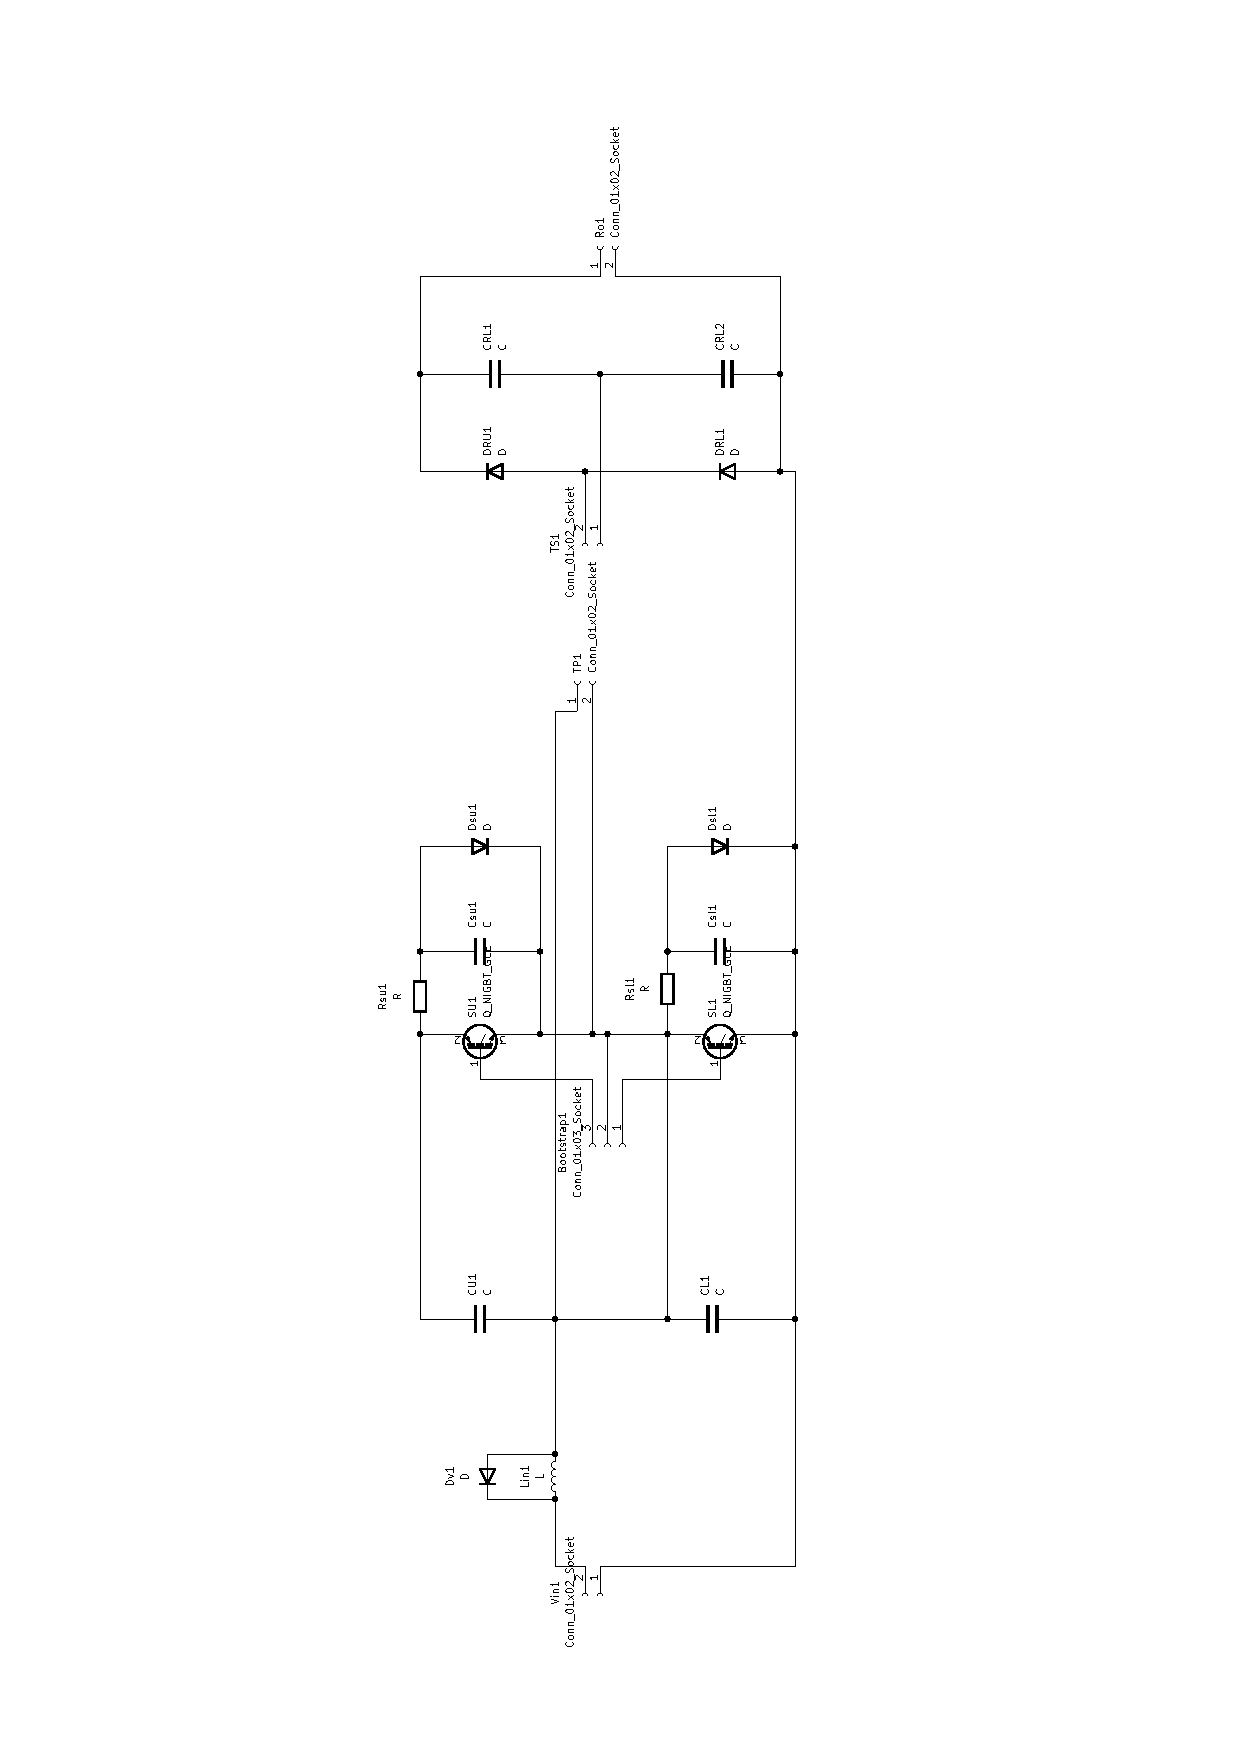
\includegraphics[width=0.8\linewidth]{img/diseño}
	\caption{Esquemático del circuito implementado.}
	\label{fig:diseno}
\end{figure}

Y, se tiene la siguiente vista de la ventana de edición de la PCB.

\begin{figure}
	\centering
	\includegraphics[width=1\linewidth]{img/pcb_edit}
	\caption{Vista de la ventana de edición de PCB en KiCAD.}
	\label{fig:pcbedit}
\end{figure}

Finalmente, el modelo en 3D de la placa a implementar es el siguiente.

\begin{figure}
	\centering
	\includegraphics[width=0.8\linewidth]{img/pcb3D}
	\caption{Vista en tres dimensiones de la placa a implementar físicamente.}
	\label{fig:pcb3d}
\end{figure}

\clearpage

\section{Conclusiones}

Este apartado se divide en dos secciones, de modo de simplificar la distinción entre puntos de vista aplicados al desarrollo del trabajo práctico.

\subsection{Técnicas}

\begin{itemize}
	\item Se completó el diseño del circuito de forma exitosa, logrando las especificaciones de diseño solicitadas, junto con las impuestas por el diseñador.
	\item Se logró una regulación de un $2.25\%$, lo que implica que se tiene una salida de tensión prácticamente constante, incluso para grandes variaciones de carga en el circuito de salida. 
	\item El tiempo de establecimiento del circuito, incluso para variaciones de carga, siempre se mantiene por debajo de los $0.5 \ ms$, lo que implica que el transitorio es muy corto, permitiendo alimentar cargas desde un inicio, antes del arranque. Relacionado a esto, también es posible mencionar el hecho de que el sobrepasamiento de la respuesta del circuito se mantiene en valores comedidos (alrededor del $5\%$), eliminando riesgos para la conexión de una carga.
\end{itemize}

\subsection{Personales}

\begin{itemize}
	\item La conclusión de la materia con un trabajo de esta magnitud es considerada un gran aporte, dado que es necesario aplicar distintos conceptos aprendidos, como: selección de componentes, criterios de diseño, intepretación de formas de onda, cálculos, análisis de resultados, entre otros.
	\item El circuito solicitado (convertidor semipuente boost compacto) consta de la implementación de varios conceptos vistos a lo largo de la materia, así como de otros no tan profundizados. Esta topologia no se encuentra correctamente explicada en mucha bibliografía por internet, lo que hizo que se haya necesitado ver fuentes confiables. Esto último permitió también, más allá del esfuerzo que requiere el diseño, un ejercicio de búsqueda de bibliografía confiable, considerado muy productivo por parte del alumno.
\end{itemize}


\clearpage
%\bibliography{library}

\begin{thebibliography}{9}
	
	\bibitem{krupa20XX}
	Krupa, Adam,
	\textit{Simulation studies of half-bridge isolated DC/DC boost converter},
	2014.
	
	\bibitem{sngate20XX}
	SN electronics,
	\textit{Considerations on bootstrap circuitry for gate drivers},
	Technical Report AN5789, 2022.
	
	\bibitem{sayed20XX}
	Sayed, Khairy,
	\textit{Boost-Half Bridge Single Power Stage PWM DC-DC Converter for Small Scale Fuel Cell Stack},
	2006.
	
	\bibitem{faizan20XX}
	Faizan, Muhammad, Wang, Xiaolei, and Yousaf, Muhammad Zain,
	\textit{Design and Comparative Analysis of an Ultra-Highly Efficient, Compact Half-Bridge LLC Resonant GaN Converter for Low-Power Applications},
	2023.
	
\end{thebibliography}

\clearpage


% ------------------------------------------------------------------------------
% ANEXO
% ------------------------------------------------------------------------------
\begin{appendixd}
	
	
	\section{Script para simular con Python}
	
	\begin{sourcecode}{python}{Código de simulación del sistema con Python.}
	# Import necessary libraries
	import xmlrpc.client as xml  # For XML-RPC server communication
	import matplotlib.pyplot as plt  # For plotting graphs
	import numpy as np  # For numerical operations
	
	# Connect to the PLECS XML-RPC server
	model = 'simulation_modif'  # Define the model name
	file_type = '.plecs'  # Define the file type
	plecs = xml.Server('http://localhost:1080/RPC2').plecs  # Create a server object
	
	# Set the plotting style
	plt.style.use('seaborn-v0_8-deep')  # Use a specific style for the plots
	
	# Simulate the model and retrieve values and time
	values = plecs.simulate(model)['Values']  # Get simulation values
	time = plecs.simulate(model)['Time']  # Get simulation time
	
	# Plot trigger signals over time
	plt.figure(figsize=(10,5))
	plt.plot(time,values[2],linewidth=2, label='Señal de disparo $S_U$')  # Upper trigger signal
	plt.plot(time,values[3],linewidth=2, label='Señal de disparo $S_L$')  # Lower trigger signal
	plt.xlabel('Tiempo (s)')
	plt.ylabel('Tensión de disparo (V)')
	plt.title('Señales de disparo en función del tiempo')
	plt.legend()
	plt.xlim(0,0.00004)
	plt.grid(True)
	plt.savefig('disparo.pdf')  # Save the plot as a PDF file
	
	# Plot primary and secondary winding voltages over time
	plt.figure(figsize=(10,10))
	plt.subplot(2,1,1)
	plt.plot(time,values[4],linewidth=2)  # Primary winding voltage
	plt.ylabel('Tensión (V)')
	plt.xlabel('Tiempo (s)')
	plt.title('Tensión del devanado primario en función del tiempo')
	plt.grid(True)
	plt.xlim(1.0860e-1,1.0865e-1)
	plt.subplot(2,1,2)
	plt.plot(time,values[6],linewidth=2)  # Secondary winding voltage
	plt.ylabel('Tensión (V)')
	plt.xlabel('Tiempo (s)')
	plt.title('Tensión del devanado secundario en función del tiempo')
	plt.grid(True)
	plt.xlim(1.0860e-1,1.0865e-1)
	plt.savefig('tensiones_transformador.pdf')  # Save the plot as a PDF file
	
	plt.figure(figsize=(10,10))
	plt.subplot(2,1,1)
	plt.plot(time,values[5],linewidth=2)
	plt.ylabel('Corriente (A)')
	plt.xlabel('Tiempo (s)')
	plt.title('Corriente en el devanado primario en función del tiempo')
	plt.grid(True)
	plt.xlim(8.14e-3,8.2e-3)
	plt.subplot(2,1,2)
	plt.plot(time,values[7],linewidth=2)
	plt.ylabel('Corriente (A)')
	plt.xlabel('Tiempo (s)')
	plt.title('Corriente en el devanado secundario en función del tiempo')
	plt.grid(True)
	plt.xlim(8.14e-3,8.2e-3)
	plt.savefig('corrientes_transformador.pdf')
	
	plt.figure(figsize=(10,10))
	plt.subplot(2,1,1)
	plt.plot(time,values[0],linewidth=2)
	plt.ylabel('Tensión (V)')
	plt.xlabel('Tiempo (s)')
	plt.title('Tensión de salida para $R_o=100\Omega$')
	plt.grid(True)
	plt.subplot(2,1,2)
	plt.plot(time,values[1],linewidth=2)
	plt.ylabel('Corriente (A)')
	plt.xlabel('Tiempo (s)')
	plt.title('Corriente de salida para $R_o=100\Omega$')
	plt.grid(True)
	plt.savefig('informe/informe_TFI/img/salida_100.pdf')
	
	plt.figure(figsize=(10,5))
	plt.plot(time,values[0],linewidth=2)
	plt.ylabel('Tensión (A)')
	plt.xlabel('Tiempo (s)')
	plt.title('Transitorio de tensión de salida para $R_o=100\Omega$')
	plt.grid(True)
	plt.xlim(0,4e-3)
	plt.savefig('informe/informe_TFI/img/transitorio.pdf')
	
	voltage = np.array(values[0])
	current = np.array(values[1])
	
	plt.figure(figsize=(10,5))
	plt.plot(time,voltage*current,linewidth=2)
	plt.ylabel('Potencia (W)')
	plt.xlabel('Tiempo (s)')
	plt.title('Potencia de salida para $R_o=100\Omega$')
	plt.grid(True)
	plt.savefig('informe/informe_TFI/img/potencia.pdf')
	
	# Calculate and print the settling time
	index_40 = np.where(voltage > 40)[0][0]  # Find the index where voltage exceeds 40V
	value_90 = 0.9 * 400  # Calculate 90% of 400V
	for i in range(index_40, len(voltage)):
	if all(voltage[i:] >= value_90):
	indice_90_por_ciento = i  # Find the index where voltage stabilizes at 90% of 400V
	break
	tiempo_establecimiento = time[indice_90_por_ciento] - time[index_40]  # Calculate settling time
	print(f"El tiempo de establecimiento es {tiempo_establecimiento} segundos.")  # Print the settling time
	
	# Simulate the model for different load resistances and plot the average output voltage and current
	resistance = np.linspace(100,50000,100)  # Define a range of load resistances
	v_mean = []  # List to store average voltages
	i_mean = []  # List to store average currents
	
	import time as t  # Import time module for sleep function
	
	for r in resistance:
	plecs.set(model+'/Ro','R',str(r))  # Set the load resistance
	values = plecs.simulate(model)['Values']  # Simulate the model
	half = len(values[0])//2  # Find the midpoint of the simulation
	half_values = values[0][half:]  # Consider values after the midpoint
	v_mean.append(np.mean(half_values))  # Calculate and store the average voltage
	i_mean.append(np.mean(values[1][half:]))  # Calculate and store the average current
	t.sleep(1e-3)  # Short pause between simulations
	
	# Plot the average output voltage and current as a function of load resistance
	plt.figure(figsize=(10,10))
	plt.subplot(2,1,1)
	plt.plot(resistance,v_mean,linewidth=2)  # Plot average voltage
	plt.ylabel('Tensión (V)')
	plt.xlabel('Resistencia de carga ($\Omega$)')
	plt.title('Tensión media de salida en función de la resistencia de carga')
	plt.grid(True)
	plt.subplot(2,1,2)
	plt.plot(resistance,i_mean,linewidth=2)  # Plot average current
	plt.ylabel('Corriente (A)')
	plt.xlabel('Resistencia de carga ($\Omega$)')
	plt.title('Corriente media de salida en función de la resistencia de carga')
	plt.grid(True)
	plt.savefig('informe/informe_TFI/img/salida_regulacion.pdf')  # Save the plot as a PDF file
	
	plt.figure(figsize=(10,10))
	plt.subplot(2,1,1)
	plt.plot(time,values[8],linewidth=2)
	plt.ylabel('Tensión (V)')
	plt.xlabel('Tiempo (s)')
	plt.title('$V_{CE}$ para IGBT en función del tiempo')
	plt.grid(True)
	plt.xlim(1.0860e-1,1.0865e-1)
	plt.subplot(2,1,2)
	plt.plot(time,values[9],linewidth=2)
	plt.ylabel('Corriente (A)')
	plt.xlabel('Tiempo (s)')
	plt.title('$I_{C}$ para IGBT en función del tiempo')
	plt.grid(True)
	plt.xlim(1.0860e-1,1.0865e-1)
	plt.savefig('informe/informe_TFI/img/signal_IGBT.pdf')
	
	plt.figure(figsize=(10,5))
	plt.plot(time,values[11],linewidth=2)
	plt.ylabel('Corriente (A)')
	plt.xlabel('Tiempo (s)')
	plt.title('Corriente en el diodo snubber')
	plt.grid(True)
	plt.xlim(2.75e-1,2.753e-1)
	plt.savefig('informe/informe_TFI/img/diodo_snubber.pdf')
	
	plt.figure(figsize=(10,10))
	plt.subplot(2,1,1)
	plt.plot(time,values[13],linewidth=2)
	plt.ylabel('Tensión (V)')
	plt.xlabel('Tiempo (s)')
	plt.title('$V_{D}$ para diodo de salida en función del tiempo')
	plt.grid(True)
	plt.xlim(1.0860e-1,1.0865e-1)
	plt.subplot(2,1,2)
	plt.plot(time,values[12],linewidth=2)
	plt.ylabel('Corriente (A)')
	plt.xlabel('Tiempo (s)')
	plt.title('$I_{F(av)}$ para diodo de salida en función del tiempo')
	plt.grid(True)
	plt.xlim(1.0860e-1,1.0865e-1)
	plt.savefig('informe/informe_TFI/img/diodo_salida.pdf')
	
	\end{sourcecode}
	
	\section{Simulación del circuito completo}
	
	Se ve en la siguiente figura el circuito completo. Arriba la topología implementada, ya mostrada anteriormente, y abajo los 10 bloques utilizados representando cada convertidor en paralelo.
	
	\begin{figure}
		\centering
		\includegraphics[width=1\linewidth]{img/schematic_com}
		\caption{Circuito implementado completo.}
		\label{fig:schematiccom}
	\end{figure}
	
	Para la máxima carga, las formas de onda de corriente y tensión son las siguientes.
	
	\begin{figure}
		\centering
		\includegraphics[width=1\linewidth]{img/salida_completa}
		\caption{Formas de onda de tensión y corriente de salida para el convertidor a máxima carga.}
		\label{fig:salidacompleta}
	\end{figure}
	
	Y, finalmente la potencia de salida es la siguiente.
	
	\begin{figure}
		\centering
		\includegraphics[width=1\linewidth]{img/potencia_completa}
		\caption{Forma de onda de potencia de salida para el convertidor a máxima carga.}
		\label{fig:potenciacompleta}
	\end{figure}
	

\end{appendixd}